% !!!!!!!!!!!!!!!!!!!!!!!!!!!!!!!!!!!!!!!!!!!!!!!!!!!!!!!!!!!!!!!!!!!!!!!!!!!!
%                                                                            !
% Adapt this file so that you can use it for your thesis					 !
%                                                                            !
% !!!!!!!!!!!!!!!!!!!!!!!!!!!!!!!!!!!!!!!!!!!!!!!!!!!!!!!!!!!!!!!!!!!!!!!!!!!!


\documentclass{micro-econ-thesis}
\usepackage{graphicx}
\usepackage{setspace}
\usepackage{float}
\usepackage[utf8]{inputenc} % depends on the font encoding that you are using

% For formatting of your bibliography, please use the following package with options 
\usepackage[style=authoryear]{biblatex}
\usepackage{gensymb}

\addbibresource{bibliography.bib} % add a bib-reference file

\begin{document}
% ----------------------------------------------------------------------------
% Details for the titlepage
% ----------------------------------------------------------------------------
\thesisTitle{Develeopment of Analysis Techniques for dynamic magnetic resonance imaging}
\thesisType{Master Thesis} % 'Master Thesis' or 'Seminar Paper'
\thesisAuthor{Aayush Nepal}
\thesisMail{aayush.nepal@uni-jena.de}
\thesisGrade{Master of Science in Medical Photonics} % leave empty for seminar papers
\thesisTutora{Prof. Dr. rer. nat. med. habil. Jürgen Reichenbach}
\thesisTutorb{Dr. rer. nat. Martin Krämer}
\thesisMatrikel{198683}
\thesisAddress{Schützenggase 2\\[.5ex]
								99423 Weimar}
\thesisDate{\today}
% In case of external supervisor
\thesisCompany{}

% Print titlepage
\thesisMakeTitle

% ----------------------------------------------------------------------------
% Abstract
% ----------------------------------------------------------------------------
\cleardoublepage
\pagenumbering{roman}
\pagestyle{plain}
%\thispagestyle{empty}
\subsection*{Abstract}
Short summary of your thesis (max. 250 words) \ldots

\clearpage
\subsection*{Acknowledgements}
If you want to thank anyone (optional) \ldots

% ----------------------------------------------------------------------------
% Table of contents
% ----------------------------------------------------------------------------
\cleardoublepage
%\thispagestyle{empty}
\tableofcontents

% ----------------------------------------------------------------------------
% List of figures/tables
% ----------------------------------------------------------------------------
\cleardoublepage
\phantomsection
\addcontentsline{toc}{section}{List of Figures}
\listoffigures
% --------------------------
\cleardoublepage
\phantomsection
\addcontentsline{toc}{section}{List of Tables}
\listoftables
% --------------------------

\cleardoublepage
\phantomsection
\addcontentsline{toc}{section}{List of Acronyms}
\section*{List of Acronyms}
\begin{tabular}{@{}ll}
FSU Jena & Friedrich-Schiller-Universität Jena\\
\end{tabular}

% --------------------------

% ----------------------------------------------------------------------------
% Contents
% ----------------------------------------------------------------------------
\cleardoublepage
\pagestyle{headings}
\pagenumbering{arabic}
\setcounter{page}{1}
% Contents
\onehalfspacing % for linespacing 1.5, you can turn it off with \singlespacing, e.g. for quotes or tables with multiline cells


\section{Introduction}
\label{sec:intro}


\subsection{The Knee }
The knee, a pivotal structure in the human body, plays an essential role in locomotion. Additionally, it functions to control the center of body mass and posture in the activities of daily living by facilitating a wide range of movements. As such, the knee's health and integrity are vital for overall quality of life, influencing everything from basic mobility to participation in complex sports. In a comprehensive survey across 15 European countries and Israel, it was found that knee pain was the third most commonly reported location of chronic pain, highlighting the significant concern it poses to public health \parencite{breivik_survey_2006}. Furthermore, arthritis/osteoarthritis (OA) was identified as the most common cause of this pain. 

And this situation has not improved with time. In Germany for instance, a recent retrospective study has found that the number of patients with OA is steadily rising \parencite{obermuller_epidemiology_2024}. 
Part of the reason knee-related issues are so prevalent and impactful is the inherent complexity of the knee joint itself. As a hub of various anatomical structures working in unison, the knee supports a range of movements and bears significant loads, making it susceptible to a variety of injuries and conditions.
Understanding the anatomy of the knee is the first step in tackling this problem. 

\textbf{Anatomy and Function}

The knee joint is the largest and the most superficial synovial joint in the body. \parencite{dalley_moores_2023}. 
It comprises three primary articulations:two femorotibial articulations (see Figure \ref{fig:rightkneeplate519}) and one femoropatellar articulation. These articulations, illustrated in figures \ref{fig:rightkneeplate519} and \ref{fig:patellarsurface}, are defined by their complexity and incongruence, features that are crucial for the joint's biomechanical performance. 
 
\begin{figure}[H]
	\centering
	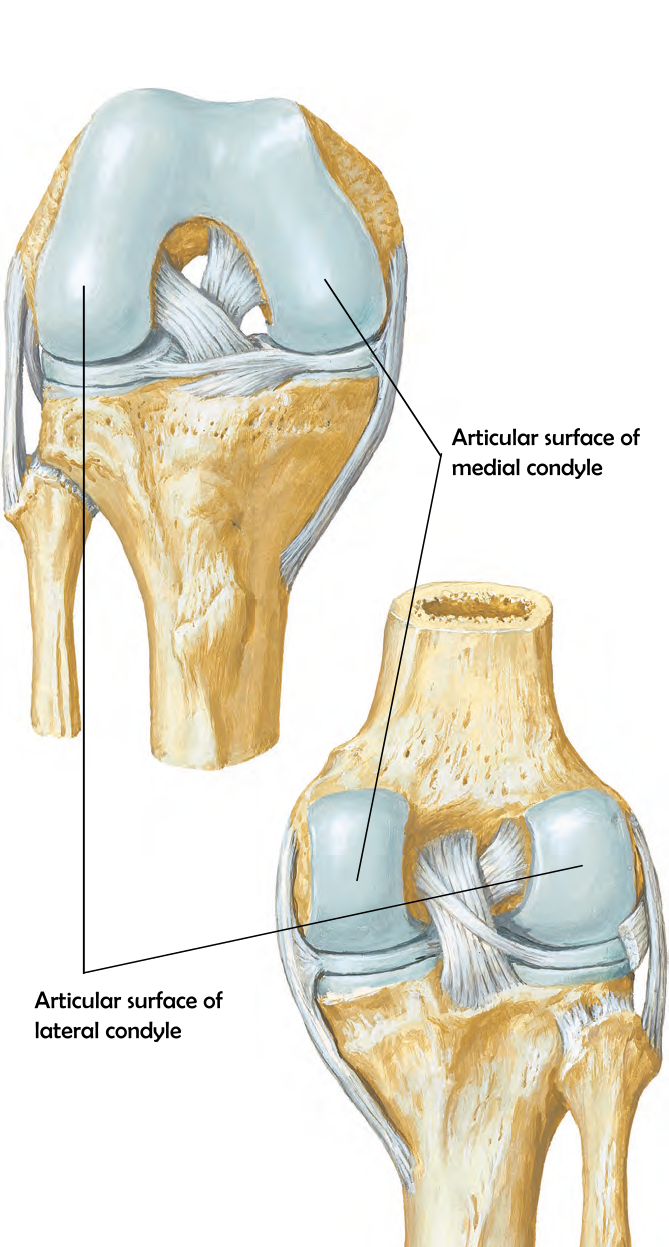
\includegraphics[width=0.7\linewidth]{right_knee_labeled}
	\caption{Anterior (flexed,top) and posterior (extended, bottom) view of the right knee with their articular surfaces labeled. \parencite[p.519]{netter_519_2023}}
	\label{fig:rightkneeplate519}
\end{figure}

\begin{figure} [H]
	\centering
	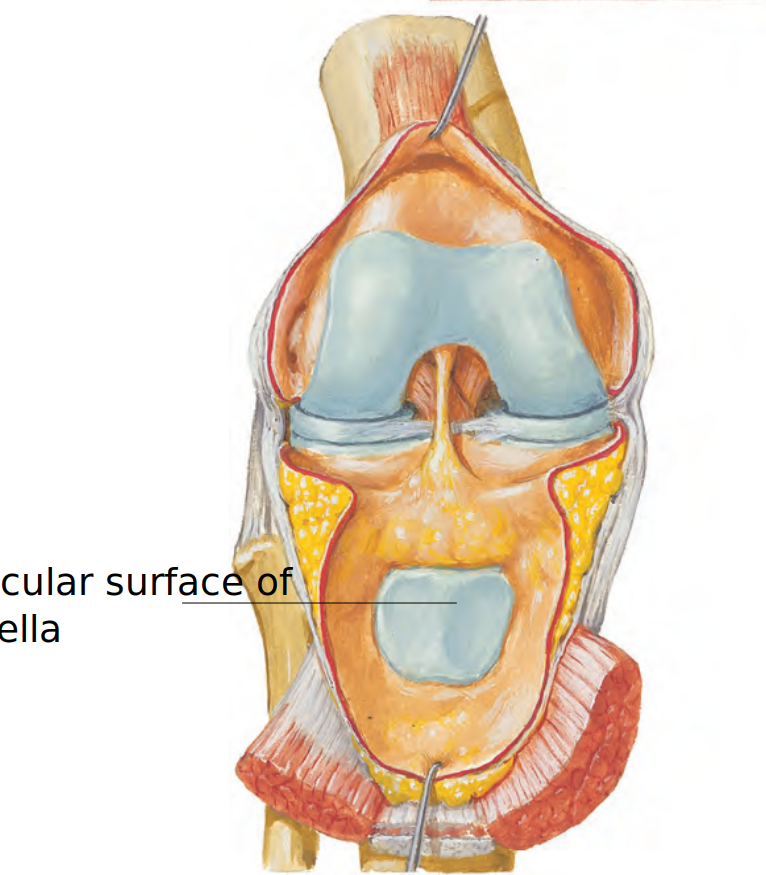
\includegraphics[width=0.7\linewidth]{patellar_surface}
	\caption[patellar surface]{Right joint opened, knee slightly in flexion, with the patellar articulation labelled. \parencite[p.517]{netter_519_2023}}
	\label{fig:patellarsurface}
\end{figure}

This design allows the knee to manage a wide array of movements and bear significant loads. Figure \ref{fig:sixdegrees} illustrates the knee's capacity for multidimensional movement, highlighting the joint's sophisticated structural design that enables this versatility. However, this inherent design also renders the knee vulnerable to a range of forces \parencite{standring_grays_2021}.

Such mechanical forces, influenced by activities and body mass index (BMI), are significant causes of OA and represent one of the most modifiable risk factors \parencite{heidari_knee_2011}. Furthermore, abnormal joint loading is considered a key mechanical driver of osteochondral changes thought to contribute to the initiation and progression of knee OA \parencite{coburn_immediate_2023}.

\begin{figure}[H]
	\centering
	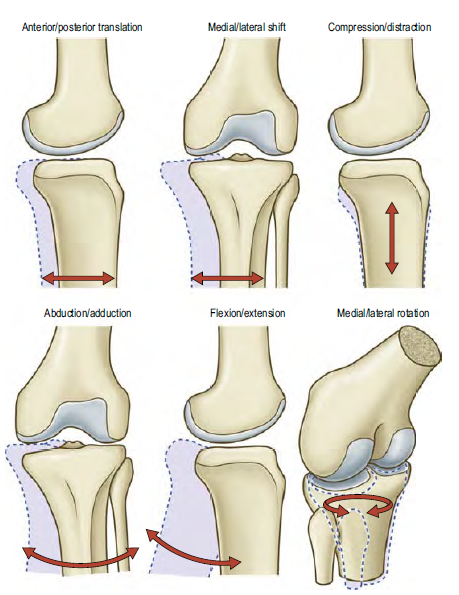
\includegraphics[width=0.7\linewidth]{six_degrees}
	\caption{The knee joint motion in three dimensions, described using six independent variables (degrees of freedom) \parencite[p.~1412]{standring_grays_2021}.}
	\label{fig:sixdegrees}
\end{figure}

The relationship between biomechanical stresses and knee health highlights the need for diagnostic tools that fulfill two key criteria: they must capture the knee's dynamic behavior during motion and assess the joint under varying loads. Dynamic magnetic resonance imaging (MRI) excels in meeting these requirements as one of the most advanced imaging modalities.

\subsection{Dynamic MRI}
In a broad sense, dynamic MRI is an umbrella term encompassing various MRI techniques designed to capture and visualize physiological processes and motion over time. This dynamic aspect of MRI is crucial when studying systems or structures where motion is inherent, such as blood flow, tissue perfusion, or cardiac movement. For the purposes of this project, the focus of "dynamic MRI" narrows down to capturing the bulk movement of the knee joint undergoing active flexion extension cycles inside the scanner. Compared to traditional static MRI scans, which are highly susceptible to motion artifacts compared to other imaging modalities \parencite{zaitsev_motion_2015}, dynamic MRI techniques not only accommodates motion, but can even leverage it to offer comprehensive insights into the functional and biomechanical properties of the concerned structures.  Among these techniques, CINE imaging, particularly renowned in cardiac MRI, is considered the gold standard for evaluating cardiac function \parencite{menchon-lara_reconstruction_2019}. This high regard in cardiac MRI illustrates the method's precision and adaptability, traits we leverage for knee imaging.

\subsubsection{CINE imaging}

CINE is derived from the word cinematography, to create a movie. In the context of dynamic knee MRI, this technique can be used to reconstruct a "movie" of a single flexion-extension cylce. This visualization is achieved by aggregating multiple partial datasets acquired over various cycles. The knee's movement cycle is segmented into distinct stages, each corresponding to a specific angle of flexion or extension. For each stage, k-space — the Fourier transform space from which MR images are reconstructed — is incrementally sampled. This data is gathered across multiple repetitions of the movement cycle, ensuring comprehensive coverage of k-space and thus, high-resolution imaging of each movement phase.This technique works robustly only if the cycles are sufficiently similar \parencite{curtis_primer_2022}. Achieving this consistency in dynamic MRI of the knee, where natural variations in movement can be significant, requires precise synchronization of the imaging process.

\subsubsection{Gating} 

This synchronization, known as gating, aligns image acquisition with specific, repeatable points in the knee's movement cycle. By ensuring each captured image corresponds accurately to a consistent phase of motion, it minimizes the discrepancies that can arise from cycle-to-cycle variations, enhancing the reliability of bio-mechanical analyses. Although there are two types of gating, namely prospective and retrospective, it is the latter that is the standard for CINE imaging as it provides a more consistent image quality \parencite[p. 102]{edelman_clinical_1996}. In retrospective gating, the data is acquired continuously throughout the motion cycle. The data is then reordered post-acquisition into a coherent sequence that shows the knee at different positions along the motion cycle. This necessitates external information that captures the precise moment and position of the knee throughout its range of movement beyond just the raw data acquired during the MRI scan. A previously reported novel knee loading device is employed to address this, which comes with an optical sensor attachment that provides this vital information \parencite{brisson_novel_2022}. 

\subsubsection{Knee loading device }

The MR-compatible knee loading device employed in this study is illustrated in Figure \ref{fig:kneedevice}. This device allowed for a range of motion of approximately 25 to 45 degrees (subject-dependent), enabling subjects to perform knee flexion and extension cycles under both loaded and unloaded conditions. For loading, the device was equipped with compartments for weight plates and sandbags, providing a physiological load of 10 to 12 kilograms. These weights are positioned at the distal end of the device, directly influencing the mechanics of knee extension. As the subject extends the knee, they must overcome not only the natural resistance of their body weight but also the additional external load imposed by these weights. Central to this device's functionality is an optical fiber position sensor (MR338-Y10C10, Micronor, 155 Camarillo, CA, USA), which precisely  measures the ab­solute angle from 0{\degree}\,to 360\degree \, with a resolution of 0.025\degree \parencite{rickenbach_optical_2013}. This measurement capability is critical for synchronizing the knee's movement with MRI data reconstruction. 
\begin{figure} [H]
	\centering
	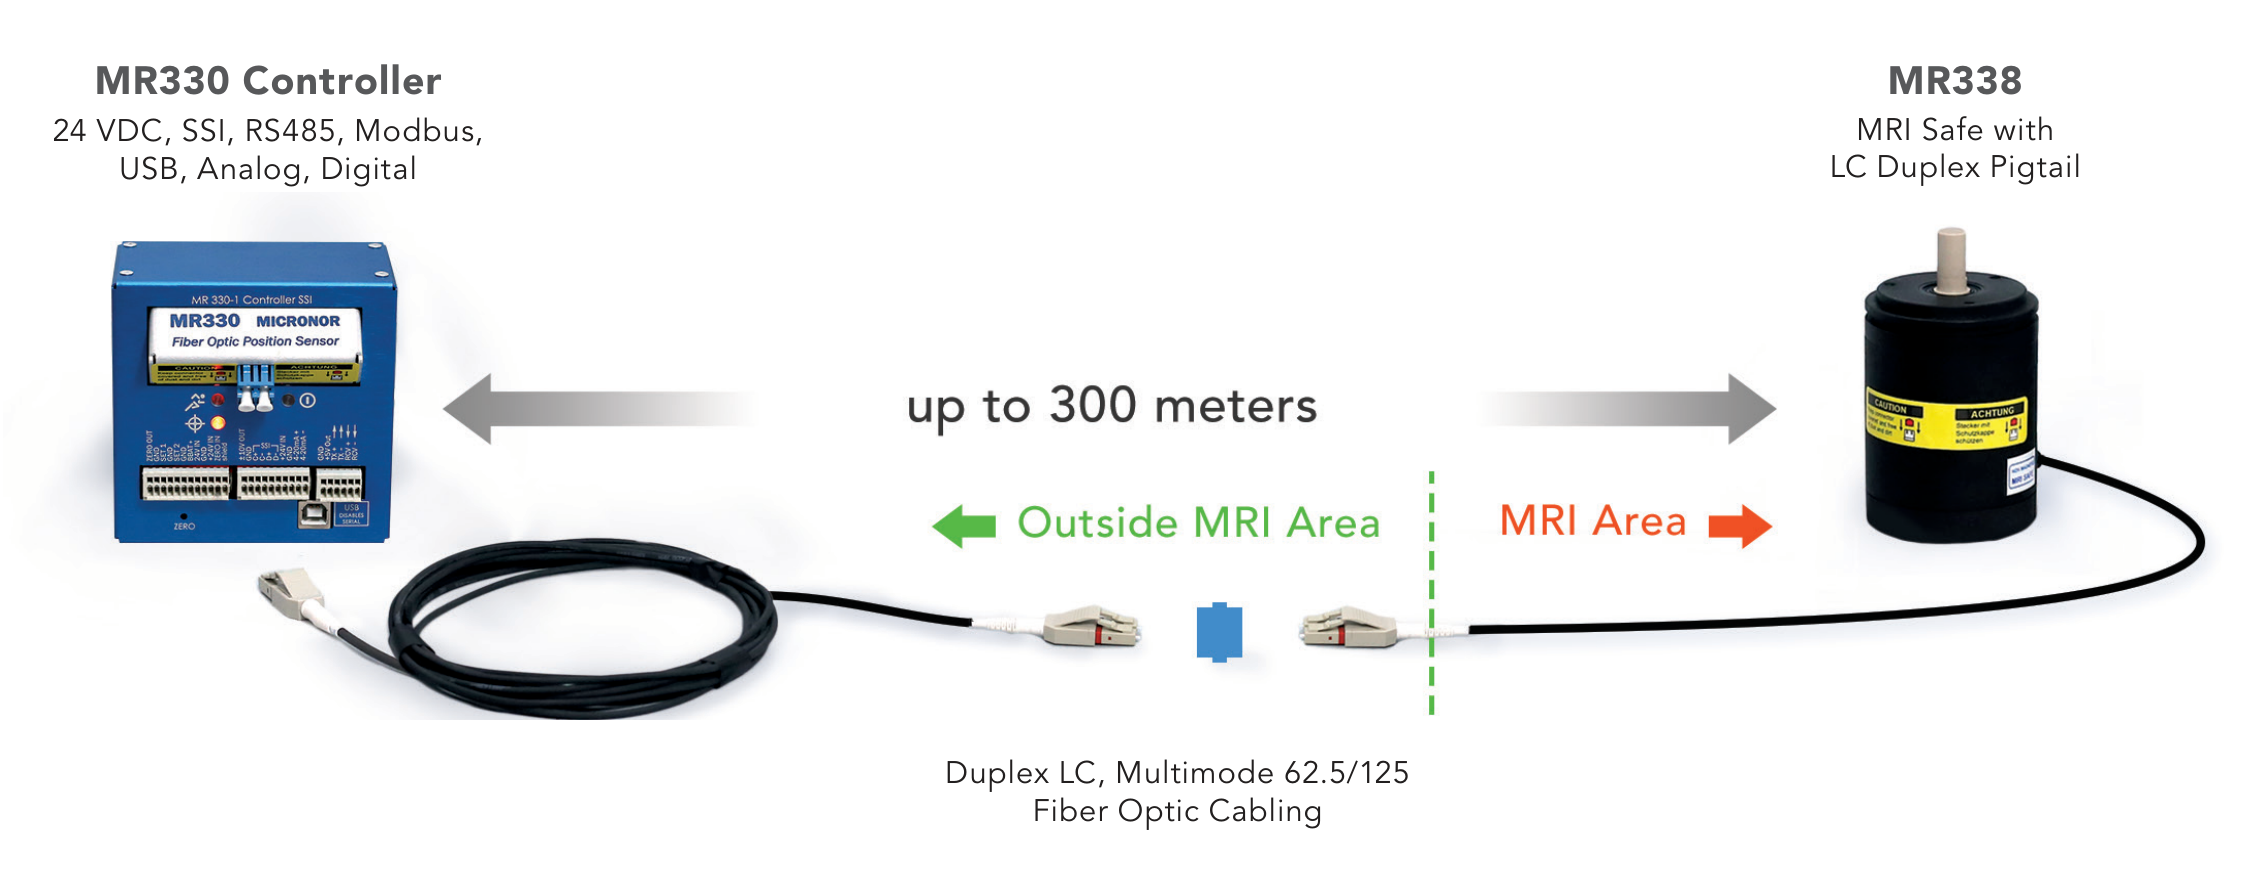
\includegraphics[width=0.7\linewidth]{sensor_img}
	\caption{The MR330 controller (left) and MR338 optical fiber position sensor system (right), showcasing the connection from the controller to the sensor via duplex LC multimode fiber optic cabling.}
	\label{fig:sensorimg}
\end{figure}


As shown in Figure \ref{fig:sensorimg} , the MR330 controller interfaces with the MRI-safe MR338 position sensor to facilitate precise measurement within the MRI environment, accommodating up to 300 meters of fiber optic cabling. The controller is connected to a laptop placed outside the scanner while the sensor is attached to the device within. To enhance signal acquisition and the clarity of imaging, two flexible coils \underline{(cite the coils here, perhaps also show a picture)} were positioned at key anatomical locations: one at the distal femur and another at the proximal tibia, as specified in the MRI protocol.
\begin{figure}[H]
	\centering
	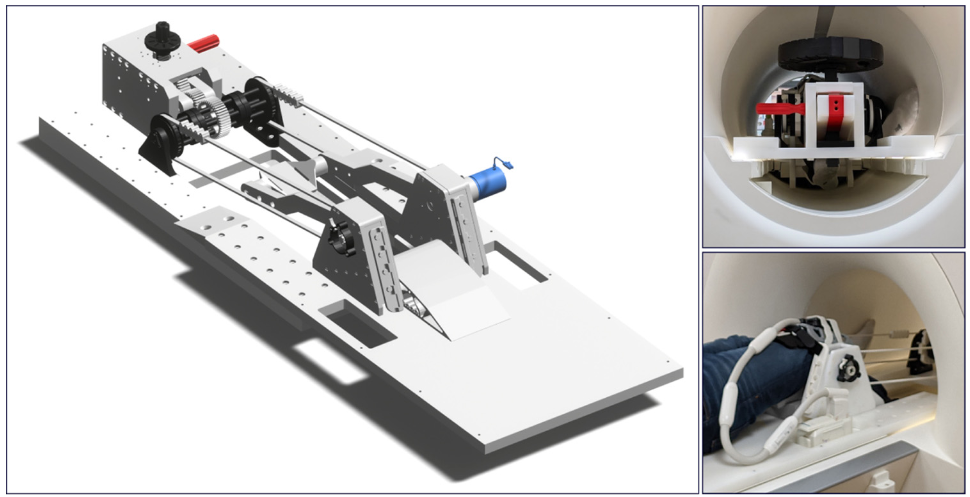
\includegraphics[width=0.9\linewidth]{knee_device}
	\caption{A 3D rendering of the knee motion/loading device (left) and two photographs of the device in a Siemens Magnetom Prisma Fit MRI scanner (right). The top right image (rear view) demonstrates how the distal part of the device sits atop the rails within the scanner bore, which are normally used to guide and support the patient table. The bottom right image (front, oblique view) demonstrates an individual positioned in the device with a flexible coil around the index knee, the thigh secured between the proximal pillow blocks and the ankle fastened to the leg support, as well as the coil plug setup.}
	\label{fig:kneedevice}
\end{figure}
 


  
To further enhance the quality and precision of our imaging, and to maximize the potential for precise image reconstruction, a previously reported radial golden-angle gradient-echo FLASH sequence was used, which is more robust against motion artifacts than Cartesian sequences \parencite{aleksiev_high-resolution_2022}. The following sections will detail the key components of this technique — radial golden-angle acquisition and the gradient-echo FLASH sequence.

\subsubsection{Radial golden-angle acquisition}


As the name suggests, radial golden-angle acquisition specifically modifies how k-space is sampled. Unlike traditional static MRI, which typically employs Cartesian sampling, this method utilizes radial sampling. Here, the data points are collected along radial lines spreading out from the center of k-space, resembling spokes on a wheel. Figure \ref{fig:radial} depicts a generic radial sampling scheme. The separation between any two adjacent circles defines the separation $\Delta k_r$ in the radial sampling direction, whereas, the angular separation between any two successive angular lines in k-space (such as between the two example lines shown in the figure) defines $\Delta \theta$. The two quantities $\Delta k_r$ and $\Delta \theta$ are constrained by the Nyquist sampling criterion. \parencite{brown_magnetic_2014} 
  
 \begin{figure}[H]
 	\centering
 	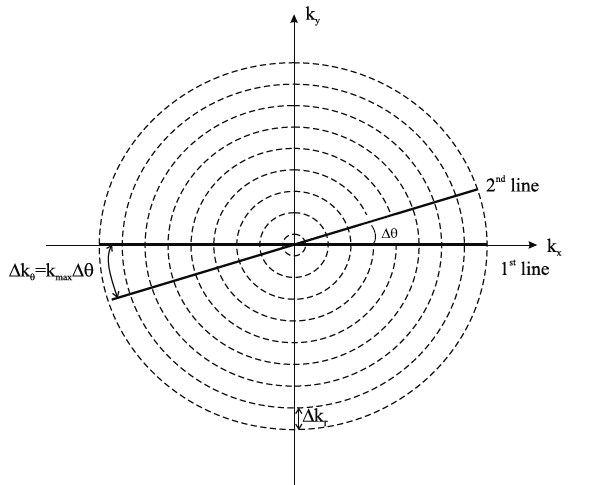
\includegraphics[width=0.7\linewidth]{radial}
 	\caption{Generic radial k-space sampling \parencite[p.306]{brown_magnetic_2014}}
 	\label{fig:radial}
 \end{figure}
 
 The 'golden-angle' strategy, which we employ, optimizes this approach by spacing the radial lines at an angle of approximately 111.25 degrees. This specific angle helps in evenly covering the k-space without overlapping, ensuring that each new image frame provides unique information, thus enhancing image quality and temporal resolution. 
 
\begin{figure}[H]
	\centering
	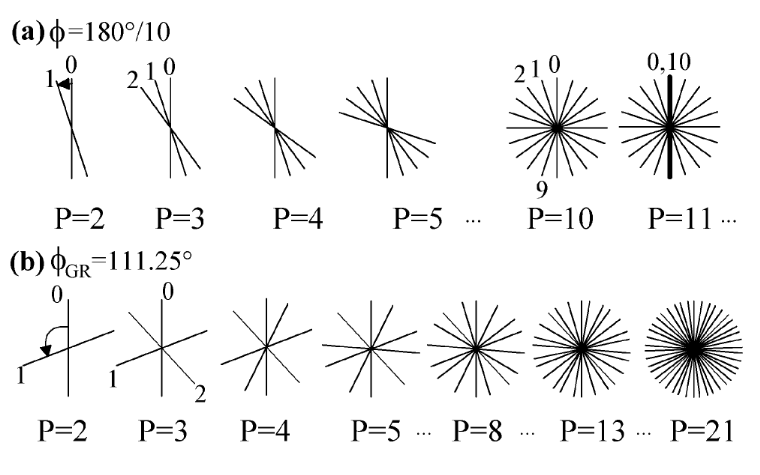
\includegraphics[width=0.7\linewidth]{golden_angle_figure}
	\caption{Radial k-space sampling strategies. (a) Fixed angular increment, showing potential for uneven k-space coverage. (b) Golden-angle sampling, ensuring uniform distribution across k-space \parencite{winkelmann_optimal_2007}.}
	\label{fig:goldenanglefigure}
\end{figure}

 
Figure \ref{fig:goldenanglefigure} provides a visual comparison between traditional fixed increment and the golden-angle methods in k-space sampling. It highlights how each approach affects the distribution of sampling lines across k-space. In the figure, part (a) shows radial sampling using a fixed angular increment. This traditional method can lead to gaps or overlaps in data collection, depending on the number of radial profiles used. Part (b) demonstrates the golden-angle method, where each new radial line is placed at an increment of approximately 111.25 degrees. This approach allows for a more uniform distribution of sampling lines across the k-space, enhancing image quality by preventing gaps and reducing redundancy in data collection. Figure blank  shows the k-space of a specific frame during the knee flexion cycle and the corresponding reconstructed MRI image.
\begin{figure}[H]
	\centering
	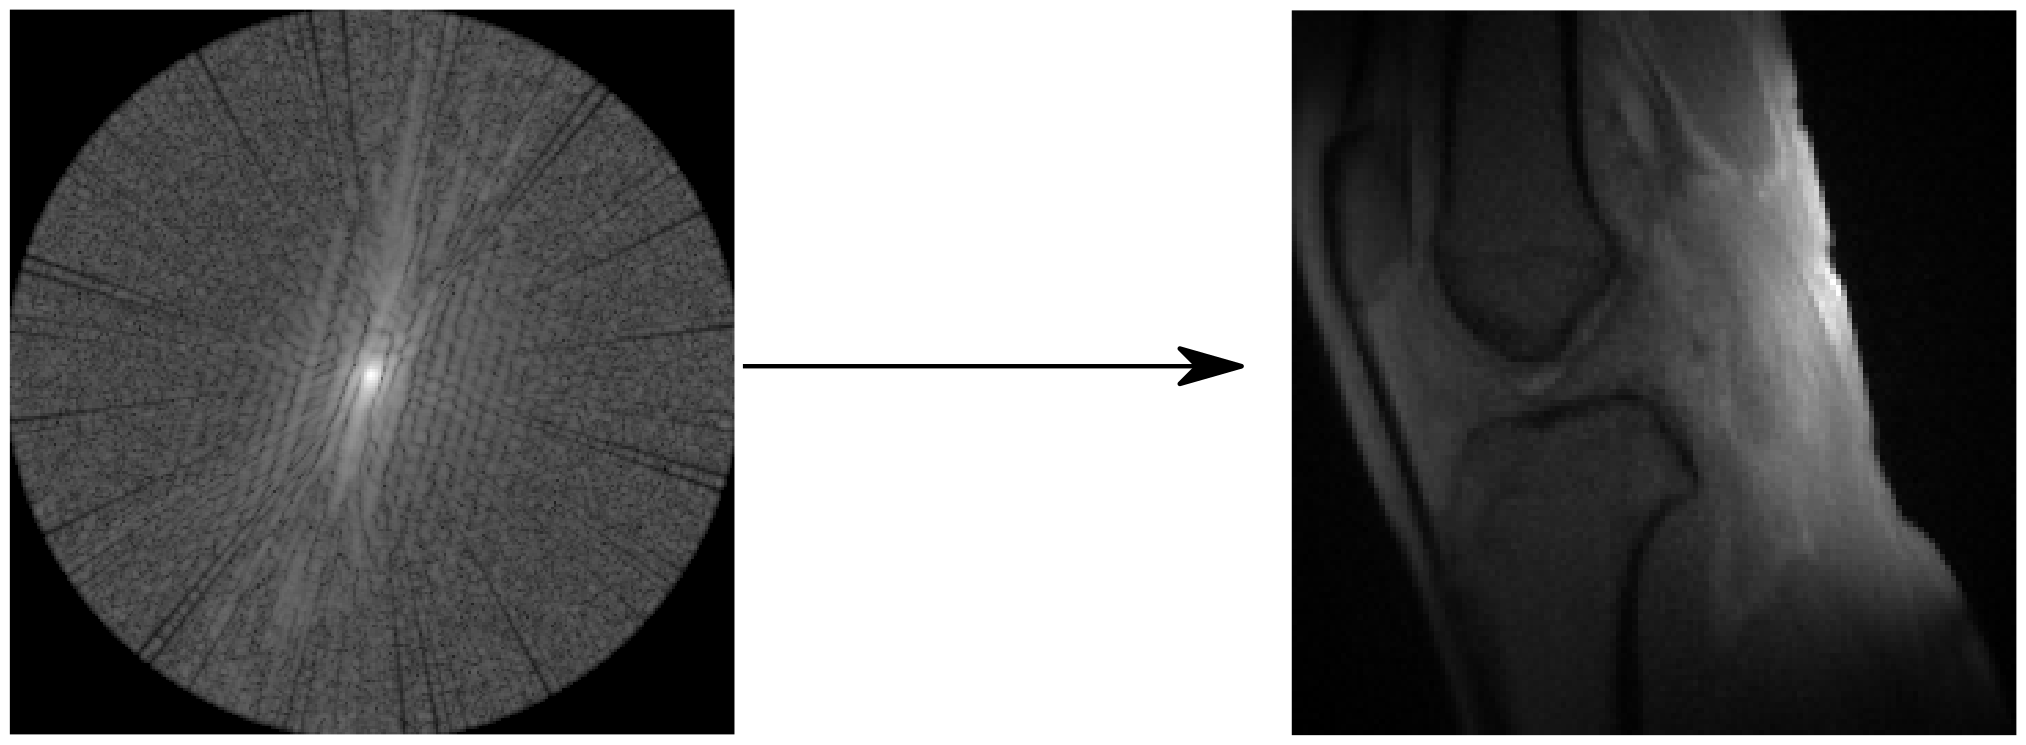
\includegraphics[width=0.9\linewidth, height=7.3cm]{kspace_arrow}
	\caption{\textbf{Example of k-space and reconstructed image}. Left: K-space data from a specific angle during the knee flexion cycle. Right: Corresponding reconstructed MRI image, illustrating the detailed visualization achievable through golden-angle sampling.}
	\label{fig:kspacearrow}
\end{figure}
  
\subsubsection{Gradient Echo FLASH sequence}

Gradient echo (GRE) is a prime candidate for dynamic MRI because it is a fast scanning process. There are two major factors that contribute to its speed. First, unlike the spin echo, we do not need to wait for a long time for the longitudinal magnetization component $M_z$ to sufficiently recover for another repetition. This is because in a GRE sequence, a smaller flip angle is used. Secondly, we do not need to wait for the spins to refocus after the application of a $180^o$ rf pulse, because there is no such pulse applied. Instead, the refocusing is done here by using magnetic field gradients of opposite polarity. The scheme of GRE sequence is depicted in Figure \ref{fig:gresimplified}. The notation is as follows: $\alpha^o$: flip angle (less than $90^o$), RF: radio frequency pulse, SS: slice selecting gradient, PE: phase encoding, FE: frequency encoding, TE: echo time and TR: repetition time. Note that in the frequency encoding direction, a negative dephasing lobe is followed by a positive gradient that brings the spins back into phase to generate the signal.    
\begin{figure}[H]
	\centering
	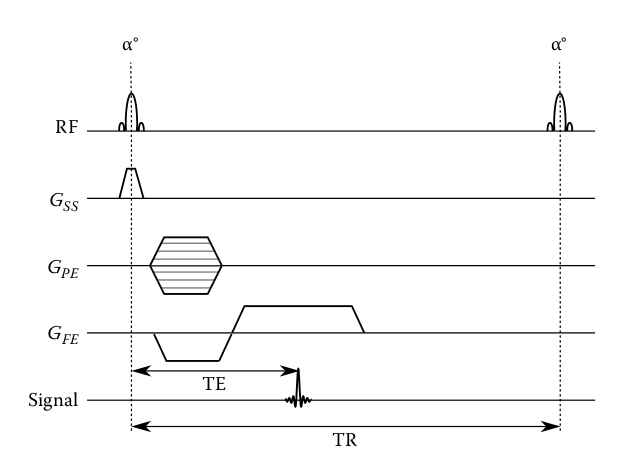
\includegraphics[width=0.7\linewidth]{gre_simplified}
	\caption{Simplified diagram of the GRE sequence that depicts the refocusing gradient applied in the frequency encoding direction \parencite[p.233]{berry_fundamentals_2009}.}
	\label{fig:gresimplified}
\end{figure}

After a series of rf pulses are delivered, we reach a condition in gradient echo sequences called the \textbf{steady state.} In this state, the magnitude of the longitudinal magnetization component $M_z$ is the same at the end of every TR. Similarly, we can also have a residual transverse magnetization $M_{xy}$ at the start of every repetition cycle. If we deliberately dephase this residual transverse magnetization, the sequence is described as incoherent or spoiled gradient echo sequences.

FLASH is a type of spoiled GRE. It is a naming scheme adopted by Siemens that spells Fast Low-Angle Shot. Other vendors have their own naming schemes for such a sequence. General Electric calls it Spoiled Gradient Echo (SPGR) and Philips calls it by the name $T_1$ fast field echo (T1-FFE). \parencite[p.583]{bernstein_handbook_2004}. The introduction of the FLASH technique in the 1980s, known for its rapid acquisition capabilities, marked a significant advancement in MRI technology. It allowed for clearer imaging of dynamic processes and reduced artifacts associated with movement. The original paper on FLASH highlights the technique's potential for 'recording NMR movies' to visualize physiological changes, a capability now fully integrated into contemporary MRI practices." \parencite{haase_flash_1986}

\subsection{Research Necessity}
With the advanced capabilities to capture high-resolution CINE MRI images of the knee during flexion-extension cycles under both loaded and unloaded conditions, we are now faced with the challenge of extracting meaningful biomechanical insights from this data. The first critical step in any such analysis typically involves segmenting the key anatomical structures within the images—namely, the femur and tibia. This process is crucial because accurate segmentation directly influences the reliability of subsequent biomechanical measurements.

Manual segmentation, while simple, is exceedingly time-consuming and susceptible to human error, highlighting the need for more efficient methodologies. In response, this thesis proposes the development of a semi-automated segmentation pipeline. This approach aims to reduce the manual effort required while maintaining high accuracy, thereby accelerating the analysis process and reducing potential biases introduced by manual methods.

Once segmentation is achieved, the next step involves measuring a biomechanical parameter-specifically, the distance between chosen anatomical landmarks on the femur and tibia. This measurement serves as an indirect indicator of joint space, which is crucial for assessing knee health. Derived from 2D images captured in the sagittal plane throughout the knee's flexion-extension cycle, this parameter allows for an analysis of how relative positions between the femur and tibia vary under different conditions of movement and load.

\subsection{Thesis Structure}
Structure of the thesis is as follows: 


\section{Methodology}
\label{sec:second}

\subsection{Data Collection Methods}

\subsubsection{Procedure Details}
Dynamic MRI scans were conducted on four healthy individuals, ranging in age from 28 to 37 years and weighing between 55 to 90 kilograms, utilizing a 3 T Siemens Prisma fit scanner. These volunteers were free from any known musculoskeletal disorders and provided their written consent, adhering to the ethical standards approved by the institutional review board. For all of these subjects, the left leg was scanned. 


Once the subject was placed supine in the scanner, the thigh was secured on a wedge positioner, and the lower leg was attached to an ankle rest, just above the malleoli, using Velcro straps to minimize lateral movement. The knee to be examined is aligned with the device’s axis of rotation, while the other leg rests alongside the MRI scanner's bore.  Knee motion is guided by a belt and sprocket assembly running alongside the lower leg, connected to a gearbox activated by the leg support as the participant flexes and extends the knee. Once the subject was positioned at the scanner's isocenter, their leg naturally assumed a flexed posture due to the design of the device. In this configuration, the leg is cradled by the device arm which is positioned below the level of the knee, ensuring that the leg remains flexed without the volunteer exerting any force.


The volunteer engaged in a controlled exercise, following a metronome set at 60 beats per minute. This pace dictates a four-beat flexion to extension cycle, with the leg being flexed at the first beat and fully extended by the fourth. This equals to 8 beats per cycle, or 7.5 cycles every minute. Initially conducted under a loaded condition with weights added to the distal end of the device, the process is repeated without the added resistance to compare both states. The scan duration is around two and a half minutes, amounting to 20 full flexion-extension-flexion cycles. 

\subsubsection{Sequence Parameters and Reconstruction}


\subsection{Data Analysis}
All the analysis and data visualization were done using the python programming language (v3.11.5). To begin, the data in nifti (Neuroimaging Informatics Technology Initiative) format is loaded using nibabel (v5.1.0) library. It is then visualized using napari(v0.4.18), a multi-dimensional interactive image viewer in Python. 
\subsubsection{Segmentation}
Step 1: Edge Detection Using the Canny Algorithm

The Canny filter \parencite{canny_computational_1986}, as implemented in the scikit-image's feature library (v0.21.0), was employed to apply an edge filter to the images. Various parameters of the Canny algorithm were adjusted, including edge thresholds and Gaussian blur, to optimize edge detection. Subsequently, the scikit-image's morphology library was utilized to remove small elements from the binary image. The image was then skeletonized to a one-pixel width, retaining only long and consistent edges. The final selection of the desired edge was accomplished using scipy's label algorithm (v1.11.3).

\subsection{Validity and Reliability}
Validation Methods: Detail the steps taken to validate the segmentation techniques and the biomechanical parameters you derived.
Reliability Measures: Describe any repeat analyses or cross-verifications done to ensure the consistency and reliability of your results.

\section{Results}
\label{sec:yetanother}

\subsection{Segmentation}
\label{subsec:last}
some text 

\subsection{Parameter Extraction}
some text 

\section{Discussion}
\subsection{Technique Evaluation}
Assess the effectiveness and accuracy of your segmentation techniques. 
\subsection{Biomechanical Insights}
Discuss the biomechanical parameters obtained and their implications for understanding knee movement. 
\subsection{Comparison with Existing Methods}
Compare your results with current analysis techniques. 
 

\section{Conclusion}
\subsection{Summary of Contributions}
Recap the novel analysis techniques developed and their significance. 
\subsection{Limitations and Challenges}
Discuss any limitations encountered and the challenges in the analysis process 
\subsection{Future Work}
Suggest potential improvements and future directions for research

% ----------------------------------------------------------------------------
% Bibliography
% ----------------------------------------------------------------------------
\cleardoublepage
\phantomsection
\addcontentsline{toc}{section}{\refname} % to add Bibliography to toc
\printbibliography

% --------------------------
\cleardoublepage
\begin{appendix}
\section{Appendix}
If needed for supplementary material, such as detailed description of data collection, tables, or figures.

\end{appendix}

% ----------------------------------------------------------------------------
% Statutory declaration
% ----------------------------------------------------------------------------
\makeThesisDeclaration

\end{document}

